\documentclass{article}
\usepackage{svg}
\usepackage{parskip}
\usepackage[most]{tcolorbox}
\usepackage{minted}
\usepackage{graphicx}
\usepackage{pdflscape}
\usepackage{xcolor}
\usepackage[
    top=0.5in,
    bottom=1in,
    left=1in,
    right=1in
]{geometry}

\begin{document}
\begin{titlepage}
    \centering
    \vspace*{\fill}

    {\Huge\bfseries Automating the Management of Software Systems\par}

     \vspace{1cm}

    \vspace*{\fill}
\end{titlepage}


\section{Introduction}
Software systems are an essential part of modern society and when they fail to function as intended, the implications can be enormous. It is therefore vital that systems are built to minimize the possibility of failure and that, when failures do occur, effective diagnostic processes expedite the systems recovery and prevent the recurrence of failures.

To address this need, this document presents a framework called the Design Learning Platform (DLP) that fully automates the diagnosis of software failures. First, I will first explore the nature of the design on its own and explain how a closed semantic world can predict and resolve failures. Next, I will talk about how the design is applied to software systems and explain the diagnostic automation that it enables. Finally, I will talk about how this framework enables the complete automation of software system management and discuss how this is practically achieved by the platform.

\section{The Design}

A design is a closed semantic world. It contains participants whose state is transformed through the design's unambiguous behaviors. When the environment interacts with the design, it introduces a change to the state of the world. This state transition may enable new behaviors, which the design deterministically resolves in response to the updated state, producing further state changes. When resolving a state, the design may either exhibit behavior directly or deterministically select which behaviors are enabled as a reaction to the state. The design continues reacting to each resulting state transition until no further behavior is enabled and the world reaches a stable semantic state. This chain of resolutions constitutes the structure of the design itself and provides the environment a fully specified path through it.

\begin{figure}[h]
    \centering
    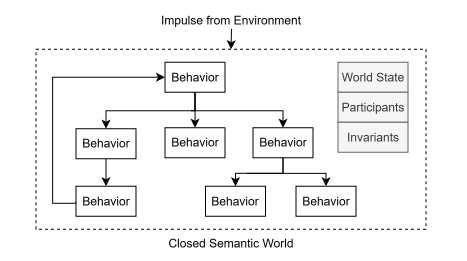
\includegraphics[width=0.8\textwidth]{../assets/design.png}
    \caption{A block diagram of the design.}
    \label{fig:the_design}
\end{figure}

The design is said to be in a semantically invalid state when one of its intentions can’t be realized as a result of the state. When the environment provides an input into this closed world, in order to continue successfully realizing its intentions, the design must prevent semantically invalid states from persisting in its reality. To achieve this, semantic invariants act as markers which identify the semantically invalid state and predict the failure of downstream behaviors. This establishes an invariant path from the semantically invalid state to the intention that can’t be realized and in order to restore semantic validity, the design must provide a semantically valid path to resolve the state.

Since the design is completely unambiguous and semantic in nature, another valid way to represent it as potential narratives within a closed semantic world and I will be using this framing in the rest of this document because it is more accessible. These narratives can be constructed by identifying the participants involved, the transformation being applied and the decisions that were made. When an environment provides an impulse into the design, a specific narrative is selected in this world. When looked at in this way, a semantically invalid path can be seen as a narrative that must be eliminated from the potential narratives of this closed semantic world and instead, the design must provide a semantically valid narrative for the environmental impulse as it moves through the design. By only allowing semantically valid narratives in the closed semantic world, the design eliminates failures with respect to all the known invariants.

\begin{figure}[h]
    \centering
    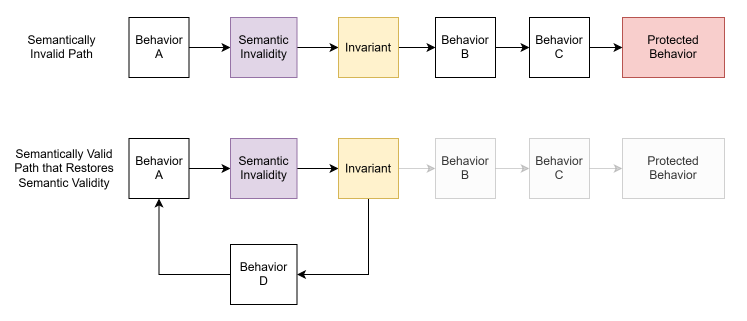
\includegraphics[width=0.8\textwidth]{../assets/invariant_path.png}
    \caption{Invariant Path}
    \label{fig:invariant_path}
\end{figure}

In the first path, since the design does not provide a semantically valid narrative for the environment, the protected behavior is reached. The failure can be automatically debugged because the failure will be predicted by the violated invariant. However, in the second path, the design does provide a semantically valid narrative to restore semantic validity and the potential bug is eliminated. Using this structure, given a semantically invalid state, the invariant can be automatically tested by walking the path and identifying if the design provides a semantically valid narrative. In this sense, it is also fair to say that semantic invariants protect the downstream behavior because they ensure that the protected behavior can never be reached through the semantically invalid narrative.

Since a design is a closed semantic world, the invariants intrinsic to the design can be identified through the control flow and data dependencies within the design's meaning. As such, the design intrinsic invariants are identified by definition and the behavior of the design can be modified to ensure that it respects every invariant and is internally consistent.If a design is tested to ensure that it respects all its known invariants and it still fails, it means that the environment which caused the failure is revealing unknown semantics that the design must learn through root cause analysis. This automates failure diagnosis because there is no other interpretation of the failure. In this process, the design becomes progressively more intelligent as it learns new semantics and invariants so that it can continue realizing its intentions in its operational environment.

In this sense, through the invariants, the design absorbs the domain knowledge needed to prevent the failures within its closed semantic world. The design itself is reshaped by the invariants to only allow semantically valid narratives to persist. In this process, by working with the design, debugging, testing and failure diagnosis are automated. However, it is clear that the diagnostic automation isn’t a result of complex analysis of the world, instead, it is the result of the world being fully constructed, resulting in unambiguous diagnosis of failures. In this sense, every time ambiguity is eliminated in a meaningful way in the closed semantic world, a new form of automation will emerge.

\section{Computable Semantic Model (CSM)}

Software systems are the result of an intentional design.The design is realized through an implementation in a programming language, which uses its abstractions to realize the design’s intentions. Therefore, the meaning behind the mechanical implementation in a programming language is established by the design of the system. Through this process of understanding the execution through the design, the automation enabled by the design is inherited by any diagnostic tool for software systems.

\begin{figure}[htbp]
    \includesvg[
        width=0.99\linewidth
    ]{../assets/computable_semantic_model.svg}
    \caption{Computable Semantic Model}
    \label{fig:computable_semantic_model}
\end{figure}

This is achieved by establishing the design as a Computable Semantic Model (CSM) in a Design Abstraction Language (DAL). A CSM is built by establishing the design structure and its transformations unambiguously in the DAL and then defining the implementation which realizes the meaning established by the design. This effectively means that the implementation exists in the context of its role in the design and any invariants specified by the implementation can be enforced by the design.

This process of establishing the design and its implementation through the CSM means that the invariants establishing the transformations correctness can reshape the permitted narratives in the world to prevent failures. It also provides a means to automatically test that the design's behavior respects the invariants specified by the transformation, effectively eliminating known failures by construction.

\subsection{Computable Semantic Primitives (CSP)}

In order for the CSM to fully automate the debugging of software systems, it is necessary for the implementation to realize the meaning of the design faithfully. If this does not happen, then it is not possible to say whether the failure occurred due to an incorrect implementation or an invariant violation. To address this, the design itself can be constructed from computable semantic primitives whose implementation can be synthesized directly from the meaning of the transformation, guaranteeing that the implementation realizes the design's meaning.

This means that the execution can be automatically debugged purely through the invariants that were violated. As later sections will explain, since it is possible to identify and eliminate semantically invalid narratives from the design, all known failures can be eliminated by construction given that the implementation faithfully realizes the design. This then automates failure diagnosis because a failure can only mean one thing, the design must learn new semantics through root cause analysis on the environment that caused the failure.

If the meaning of a behavior is opaque, by which I mean, it cannot be decomposed to computable semantic primitives, then the engines ability to reason is limited to the meaning that has been established in the world. While this isn't inherently a problem if the implementation realizes the meaning of the design, this breaks the claim of fully automated debugging. As long as the engine cannot reason about the world completely, it cannot gaurantee that all known semanitcally invalid narratives have been eliminated.

Before continuing with the larger implications of establishing software systems as computable semantic models, I will briefly discuss the Design Abstraction Language and how it enables the computable semantic model to be built.

\section{Design Abstraction Language (DAL)}

The Design Abstraction Language is a declarative language that enables the specification of closed semantic worlds. The scope of language is determined by any mechanism needed to faithfully represent the design's meaning such as the behaviors, participants attributes, control flow and invariants.

As later sections will describe, the design established through the DAL can be used by an engine to reason about the closed semantic world. Any question about the world that can’t be automatically answered must be addressed by establishing the necessary meaning through the DAL.

As the computable semantic primitives section described, when the design is built from computable semantic primitives, the implementation is directly synthesized from the design without any opaque meaning. This means that the DAL essentially becomes a declarative language that establishes the meaning of a closed semantic world and synthesizes the meaning of that world as an implementation.

\section{Shared Meaning and Distributed Systems}

One of the consequences of the computable semantic model is that the meaning behind the execution of a software system is unambiguous. As a result, software systems can achieve successful coordination through shared meaning. I will first talk about how shared meaning leads to successful interaction in a general sense and then apply it to software systems.

Imagine you visit a library, find the book you are looking for and walk up to the librarian with the intention of checking out a book. In order to check out the book, you present the librarian with the book but the librarian was expecting a library card and the interaction halts. In this case, what it means to check out a book is different for the librarian and the visitor. Since there is no shared meaning between the two, the interaction fails and neither the librarian nor the visitor achieve their goal.

In this example, since it is two humans interacting, they can clarify and establish a shared meaning and move forward with the interaction. However, software systems can't improvise(yet), so shared meaning has to be established by construction. The CSM provides the mechanism to eliminate ambiguity in the meaning of interactions between software systems through their design.

\subsection{Semantically Compatible Designs}

Consider the system shown in Figure~\ref{fig:semantically_compatible_interactions}. This example establishes a distributed image compression service that connects multiple designs together. In this example, each node is its own design. When two designs are interacting with each other, in order to successfully coordinate they must share the same meaning.

\begin{figure}[h]
    \centering
    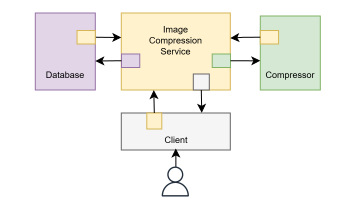
\includegraphics[width=0.8\textwidth]{../assets/semantically_valid_interaction.png}
    \caption{Semantically Compatible Interactions}
    \label{fig:semantically_compatible_interactions}
\end{figure}

When the meaning of the database is established, it also establishes the meaning of a database user. Therefore when the image compression service is interacting with the database, it takes

on the role of the database user and communicates with shared meaning. In this sense, the interaction between the two designs is semantically valid because they share the same meaning. In the diagram, I highlight this using a color scheme to indicate that each design is invoking shared meaning between both designs.

As a result, through semantically compatible interactions between designs, larger semantic worlds can be constructed. The larger semantic world establishes a new level of meaning that is defined by the semantically compatible designs that make up its reality. This frames a distributed system as a semantic world constructed from semantically compatible interactions between designs.

In order for successful interaction, the meaning that must be established on both sides of the interaction is unambiguous and this happens by design. In addition, the same principles that define the correctness of a design are equally as valid at this level of meaning. By tracking interactions between designs, environmental invariants can be identified at a particular level of meaning in the closed semantic world that represents a distributed system.

\subsection{Securing Interactions Between and Within Designs}

Finally, as a result, interaction between designs now has unambiguous meaning. There are meaningful implications for securing systems because the intention of the interaction is unambiguous. While before, the mechanical sequence had to be correct, now the design can ensure that it is the right narrative that is communicating with it. If the design is looked at as the brain of the software system, then this ensures that the correct brain is speaking, making it more difficult to compromise a system.

There are many approaches to implement this but one could be that the DAL can be extended to generate a dynamic checksum along the narrative path to identify unique narrative identity. There are more interesting ways that I can think of for securing it further by sharing the identity of the instance of the brain and using that to generate the proof. Regardless, the point here is, by eliminating ambiguity in a meaningful way, more automation will be enabled and securing the interaction between and within designs is another application for this framework.

\begin{landscape}
\begin{figure}[htbp]
\centering
\includesvg[
    width=0.99\linewidth
]{../assets/ADLP_v31.svg}
\caption{The Design Learning Platform}
\label{fig:dlp-diagram}
\end{figure}
\end{landscape}


\section{Design Learning Platform}
In this section I will discuss the Design Learning Platform as the practical framework that realizes this solution. I will also discuss how the practical hurdles faced when implementing this solution at scale are overcome.

The CSM is the mechanism through which ambiguity is eliminated in the construction of software systems. This means an engine that operates on the CSM can automatically generate the information needed for it to unambiguously understand the designs execution and enable deterministic learning. The engine does not analyze or arrive at conclusions on its own, instead, it simply enforces the correctness established by the model.

As mentioned earlier, every time that ambiguity is meaningfully eliminated from the CSM, a new form of automation emerges. In this document, I've described how the following is automated:

\begin{itemize}
    \item Failure Diagnosis: Known invariant violation or unknown invariant is identified.
    \item Debugging: Which invariant was violated?
    \item Testing: Does the design respect all known invariants?
    \item Documentation: Design written in the DAL represents itself.
\end{itemize}

Now I will talk about how the engine practically achieves the failure diagnosis, debugging and testing.

The engine is a tool that performs semantic reasoning on the constructed closed semantic world. For example, by specifying the meaning of the participants, behaviors and invariants, the design can reason about the correctness of the world. It can identify the semantically invalid narratives in the world and automatically identify how to restore semantically invalid states by establishing semantically valid narratives. The extent of its ability to semantically reason about the world is limited by the meaning established in the world.

Practically, the engine uses the invariants specified for each behavior (or computable transformation) to automatically place the invariants using the design's structure. It then uses the invariants definition to establish a semantically invalid state and it walks the invariant path to find the control flow that restores semantic validity and establishes whether it selects a semantically valid narrative. If no such control flow exists, then it concludes that the design behavior does not respect the invariant. If such a control flow does exist, it knows that the semantically invalid narrative is eliminated from the closed semantic world.

After this process, since every known failure is eliminated by construction and verified through the invariant testing, failure diagnosis is automated because an observed failure can only mean that new semantics must be learnt through root cause analysis. To achieve this, the engine automatically instruments the synthesized executable output to log the necessary information needed to replay the failed execution. This is once again possible because of the complete construction of the CSM because it unambiguously identifies all the information that can't be
deterministically reproduced. Then the failed execution of the CSM can be replayed using the logged inputs to aid in the root cause analysis.

After root cause analysis and the expansion of the semantics, the same process repeats and the design is tested to ensure that it respects the new invariant. In this way, the engine essentially tests that the design respects every invariant to automate failure diagnosis and enables deterministic learning from failures by enabling root cause analysis on the environment which reveals the new semantics. This means that the environment which reveals the new semantics must be losslessly preserved at scale. If it isn't, then the automatic and deterministic nature of this process is broken.

To address this, the design's unambiguous nature can once again be exploited to provide the domain structure of the participants. Using this structure, domain specific compression can be applied to preserve all the environments at minimal cost. Domain specific compression is a technique that exploits the known domain structure of the data to maximize its compression.

To practically achieve this, an open source tool named Compressed Log Processor (CLP) can be leveraged. It is a tool that can apply domain specific compression to the data and also search the compressed data without decompression. More importantly, it has been proven at a petabyte scale, establishing that it is possible to preserve the environments to learn new semantics through root cause analysis at scale.

CLP’s gains are achieved through the elimination of ambiguity in the domain structure of the data. Since the CSM works to eliminate any ambiguity in the construction of software systems, the compression that can be achieved by CLP is maximized. Currently CLP compresses structured and unstructured logs but this process will turn CLP into a domain specific compression engine.

Since every environment that motivated new semantics is preserved, it results in a design repository through which the evolution of the software system can be deterministically replayed. The repository tracks not just the changes to the implementation but also how the system was designed, executed and refined through learnt semantics over time.

This entire process is captured in a framework called the Design Learning Platform(DLP). It leverages the CSM and domain specific compression to fully automate the diagnosis of software failures and deterministically learn from losslessly preserved environments. In the process, it automates failure diagnosis, debugging and testing.
In the next section, I will talk about how the CSM enables automated orchestration of software systems, including deployment, recovery, upgrade and lifecycle management. Finally, I will talk about how in addition to the automation discussed so far, through the ambiguity eliminated by computable semantic models, the automation of systems management becomes fully automated because it allows the engine to semantically reason over the closed semantic world.

\section{Automating Orchestration}

In order for a design to successfully realize its intentions, the conditions necessary for it to be able to realize its intentions must exist. This can be as simple as deploying the designs onto a node, performing life cycle operations or more specific tasks like recovering from failures. As such, when the design of a distributed system is established, it also defines a manager that can successfully orchestrate the distributed system.

Orchestrating is ultimately responding to the state of the system appropriately to restore the system's ability to realize its intentions. Like with all other processes in this framework, the key to automating it is to eliminate ambiguity. Through the CSM, the meaning of a software systems state is entirely unambiguous. Each impulse into the system creates an unambiguous narrative that ripples through the system, even if it ends in failure. Since the narrative is un ambiguous, there can be an automatic unambiguous response by the management system.

Once again, this is made possible by eliminating the ambiguity in the meaning of software systems. In this case, as the impulse moves through the system, it can self-identify the narrative that it is executing, for example:

"At 9:01 AM I started when the user chose to add a book to the library. Then they submitted a book name and then I created the book. However, I failed when I attempted to read the first letter of the book's name."

The failure in this narrative won't actually happen because the invariants in the CSM would have identified it and testing would have eliminated it. However, it is a simple example to convey the idea and this extends to distributed systems naturally because the designs have shared meaning. While recovering from failures is one part of the orchestration, the same principle applies to life cycle management because the meaning of the system's state is unambiguous and the response to it is unambiguous.

\begin{figure}[h]
    \centering
    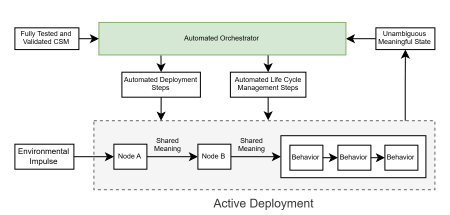
\includegraphics[width=0.8\textwidth]{../assets/AutomatedManagement.png}
    \caption{Automated Orchestration}
    \label{fig:example}
\end{figure}

This means that the manager must be designed to respond appropriately to every meaningful state in the design it is managing. Practically, it won't have to account for every narrative, instead, each design can self identify the states that will need to be managed and internally group narratives into meaningful states. Through this, an enumeration of every meaningful state can be obtained from the design and the manager can be tested to ensure that it responds appropriately.

\begin{figure}[h]
    \centering
    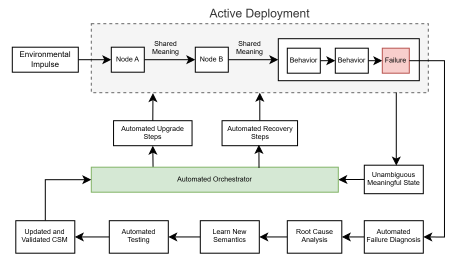
\includegraphics[width=0.8\textwidth]{../assets/AutomatedManagementFailure.png}
    \caption{Automated Failure Response}
    \label{fig:example}
\end{figure}

When a failure occurs, automated failure diagnosis is performed and the diagnostic data collected from the automated instrumentation is presented to the developer for root cause analysis to deterministically learn new semantics and prevent future failures. Once the design learns new semantics and it is automatically tested and validated, the automated orchestrator can upgrade the design with the updated CSM.

At the same time, to immediately respond to the failure and restore the system, the orchestrator automatically responds to the state of the system and takes unambiguous steps to restore the system's ability to realize its intentions.

The intelligence of the response by the orchestrator is entirely up to its design, since there is no ambiguity in the state it is responding to or the design it is managing, it can surgically recover the system to restore normal functionality or upgrade the system to deploy the updated CSM.

Ultimately, when combined with the deterministic learning loop established in earlier sections, the ability to automatically orchestrate the software system automates the processes involved in ensuring that the design's intentions can be realized in its operational environment.

In the next section I will talk about how the CSM fully automates the management of software systems by enabling automated semantic reasoning over the unambiguous world.

\section{Automating Systems Management}

In earlier sections, when discussing automated invariant placement and establishment of semantically valid narratives, I was discussing a form of semantic reasoning over the closed semantic world. While this is particularly relevant to automated failure diagnosis (through elimination of known semantically invalid narratives), ultimately, any form of reasoning over the closed semantic world can be achieved given that the necessary meaning has been established. 

Through this process, the apparent complexity of software systems will be collapsed into the clarity of a coherent design. Since the design is a closed semantic world, the ability to ask any meaningful question about that world and to be able to automatically receive meaningful answers to automate the management of that world is a very powerful capability.

For example, the engine can answer if the requirements which motivated a design are satisfied by the closed semantic world. This is possible because the requirements have shared meaning with the design and this enables the engine to automatically answer if it is satisfied. Another example could be the elimination of redundant steps in the narrative by automatically identifying if particular paths or subpaths don't have any meaningful effect on the world. These are just a few examples but the type of questions that can be asked is simply limited by the world meaning that has been established through the CSM.

This does not invent anything new, it is simply formalizing the existing software engineering process into an unambiguous and computable model so that it can be automated. The novelty of the CSM is that it has made the automation of software systems possible by enabling the engine to reason about the meaning of the closed semantic world in the same way that humans do. This is made possible by constructing the world from computable semantic primitives that eliminate the semantic gap between the implementation and the design. In this sense, this practical mechanism to automate the management of software systems is simply the logical conclusion of what was already common knowledge. 

When the CSM is used to automate the management of software systems, it is evident that through semantic reasoning and automated failure diagnosis a deterministic learning loop emerges to expand the design semantics through root cause analysis on environments that caused the failure. This is a meaningful part of fully automating systems management because the meaning of the failure is unambiguous and it results in a deterministic process that motivates the management steps. However, to enable this deterministic process at scale, every environment that caused a failure must be preserved.

To solve this problem, the unambiguous domain structure of the design is exploited in multiple ways. First, the minimal information necessary to replay the execution is unambiguously established by specifying all the information that the design cannot deterministically reproduce. Second, the unambiguous domain structure of the data is exploited to apply domain specific compression to minimize the cost of preserving the environments. To make this possible, an open source tool named Compressed Log Processor is leveraged. It has proven that domain specific compression is practical at a petabyte scale.

The novelty of CLP is that as part of the automated management, the environments that caused failures must be preserved at scale to enable the design to learn new semantics through root cause analysis. Without this, the learning loop would be broken and the management would not be automatic. Thus, by exploiting the unambiguous domain specification of the CSM, CLP enables the automation of software systems management by preserving the environments that teach the design new semantics through root cause analysis at scale.

In many ways, CLP is the real unknown mechanism to automating software systems management. While the CSM does establish functionality that didn't exist before, the actual mechanism that would make it possible was already known. However, the same could not be said about CLP and in establishing domain specific compression as an established capability, it has established a previously unknown capability that made automated software systems management practical. 

\section{Conclusion}

The techniques presented in this document take a fundamentally different approach to software systems management than existing approaches. It provides the means to complete the construction of a software system by establishing its design in a Design Abstraction Language (DAL) as a Computable Semantic Model (CSM) built from Computable Semantic Primitives (CSP) that unambiguously establishes its meaning.

This results in an engine that can automatically reason about the closed semantic world to answer any meaningful question given that the necessary meaning has been established. It treats any manual effort as a symptom of incomplete construction and provides the means to complete the construction. 

The semantic reasoning results in the automation of software failure diagnosis because it eliminates any semantically invalid narratives by construction. As a result, the environments that cause failures reveal new semantics that can be learned through root cause analysis. To enable this deterministic learning process at scale, it leverages the unambiguous nature of the CSM to preserve the environments which reveal new semantics using a tool named Compressed Log Processor (CLP) to apply domain specific compression.

Ultimately, this solution does not invent anything new. Software systems have always operated at this level of meaning and there is nothing that this solution presents that wasn't already common knowledge. What makes it novel is that it takes steps to unambiguously understand the implementation of the software system through the meaning established by its design.

This solution ultimately eliminates ambiguity in the development and maintenance of software systems. As a result, the software systems that run modern society are less likely to fail and if they do fail, an automated process ensures their recovery and automated failure diagnosis supports deterministic learning to prevent future failures. The future of software development will be less about writing bug free code and more about building intelligent and secure systems that understand each other.

\end{document}